\section{Description et justification de la solution architecturale obtenue pour le circuit}

\subsubsection*{Objectifs}

Une fois la description fonctionnelle définie, la conception passe au \textbf{niveau architectural} du diagramme en Y.  
Cette phase vise à transformer la description fonctionnelle en une organisation interne du système : 
elle introduit les interfaces physiques, identifie les ressources de stockage et de traitement, et 
établit les principes de commande et de transfert des données.

\medskip

Cette description reste indépendante de la technologie d’implémentation (langage HDL, logique, FPGA, etc.) 
mais tient compte des contraintes structurelles et temporelles du système.  
Elle correspond au \textbf{niveau Registre-Transfert (RT)}.

\begin{itemize}
    \item Introduction et définition des interfaces physiques
    \item Identification des ressources logiques (registres, compteurs, opérateurs)
    \item Organisation structurelle du circuit au niveau RT
    \item Description du comportement séquentiel et des signaux de commande
\end{itemize}

\vspace{1em}

\subsection{Horloge}

La gestion de l’horloge constitue un élément fondamental de la synchronisation interne du système.

Le rapport entre la période du bit LIN et celle du processeur est défini par :

\[
N = \frac{T_{\text{bit}}}{T_{\text{processeur}}}
\]

Dans notre cas, le cahier des charges spécifie un cycle de lecture/écriture moyen de 100~ns et une vitesse de transmission de 19\,200~bit/s, soit :

\[
N = \frac{52~\mu s}{100~ns} = 520
\]

Pour notre implémentation, nous choisissons \(N = 2048\), une valeur supérieure qui facilite la synchronisation interne et la gestion des transitions logiques.

\subsection{Architecture de la Réception de Trame}

Ce bloc correspond à la partie du système chargée de la réception et du décodage des trames LIN.

\begin{center}
\renewcommand{\arraystretch}{1.2}
\small
\begin{tabularx}{\textwidth}{|c||c|c|X|}
\hline
\textbf{Signal} & \textbf{Sens} & \textbf{Nature} & \textbf{Rôle fonctionnel} \\ \hline
LIN & Entrée & Données & Signal série reçu depuis le bus LIN \\ 
SEL\_ADR & Entrée & Données & Sélection de l’adresse du composant \\ 
DATA\_OUT & Sortie & Données & Octet de données reçu \\ 
DATA\_WR & Sortie & Commande & Validation d’écriture vers la mémoire FIFO \\ 
DATA\_RST & Sortie & Commande & Réinitialisation des données reçues \\ 
ERR\_START & Sortie & Indicateur & Erreur sur bit de start \\ 
ERR\_STOP & Sortie & Indicateur & Erreur sur bit de stop \\ 
ERR\_SYNC & Sortie & Indicateur & Erreur de synchronisation (Synchro Break) \\ 
INC\_COUNT & Sortie & Commande & Incrémentation du compteur d’octets reçus \\ 
FRAME\_VALID & Sortie & Indicateur & Trame reçue et validée \\ 
COUNT\_RST & Sortie & Commande & Réinitialisation du compteur d’octets \\ 
\hline
\end{tabularx}
\end{center}

\medskip

Le bloc de réception repose sur une \textbf{machine séquentielle} structurée en deux sous-parties :
\begin{itemize}
    \item une \textbf{unité opérative} regroupant les registres, compteurs et multiplexeurs ;
    \item une \textbf{unité de commande} gérant la séquence d’opérations et les signaux de contrôle.
\end{itemize}

\begin{figure}[H]
    \centering
    \includegraphics[width=0.8\linewidth]{images/inter/Machine_Seq_Reception_trame.pdf}
    \caption{Organisation séquentielle du bloc de réception de trame}
    \label{fig:reception_seq}
\end{figure}

Les principales variables internes assurent la gestion du comptage, du stockage et du décalage des bits reçus :

\begin{table}[h!]
    \centering
    \resizebox{\textwidth}{!}{%
        \begin{tabular}{|c|c|c|c|c|}
            \hline
            \textbf{Variable} & \textbf{Taille (bit)} & \textbf{Opération} & \textbf{Opérateur} & \textbf{Signaux de contrôle} \\ 
            \hline
            n & $\log_2(N)$ & décrémentation, initialisation à $N-1$ ou $N/2$ & décompteur, Mux & n\_Load, n\_En, n\_select \\ 
            \hline
            NbTbit & 4 & décrémentation, initialisation à 13 ou 8 & décompteur, Mux & NBTbit\_Load, NBTbit\_en, NBTbit\_select \\ 
            \hline
            Identifier & 8 & sauvegarde & registre 8 bits & Identifier\_en \\ 
            \hline
            OctetsReçus & 8 & décalage bit à bit & registre à décalage & OctetReçu\_en \\ 
            \hline
            NbDataField & 3 & décrémentation, initialisation à 1, 3 ou 7 & décompteur, décodeur & NBdatafield\_en, NBdatafield\_load \\ 
            \hline
        \end{tabular}%
    }
\end{table}



\begin{figure}[H]
    \centering
    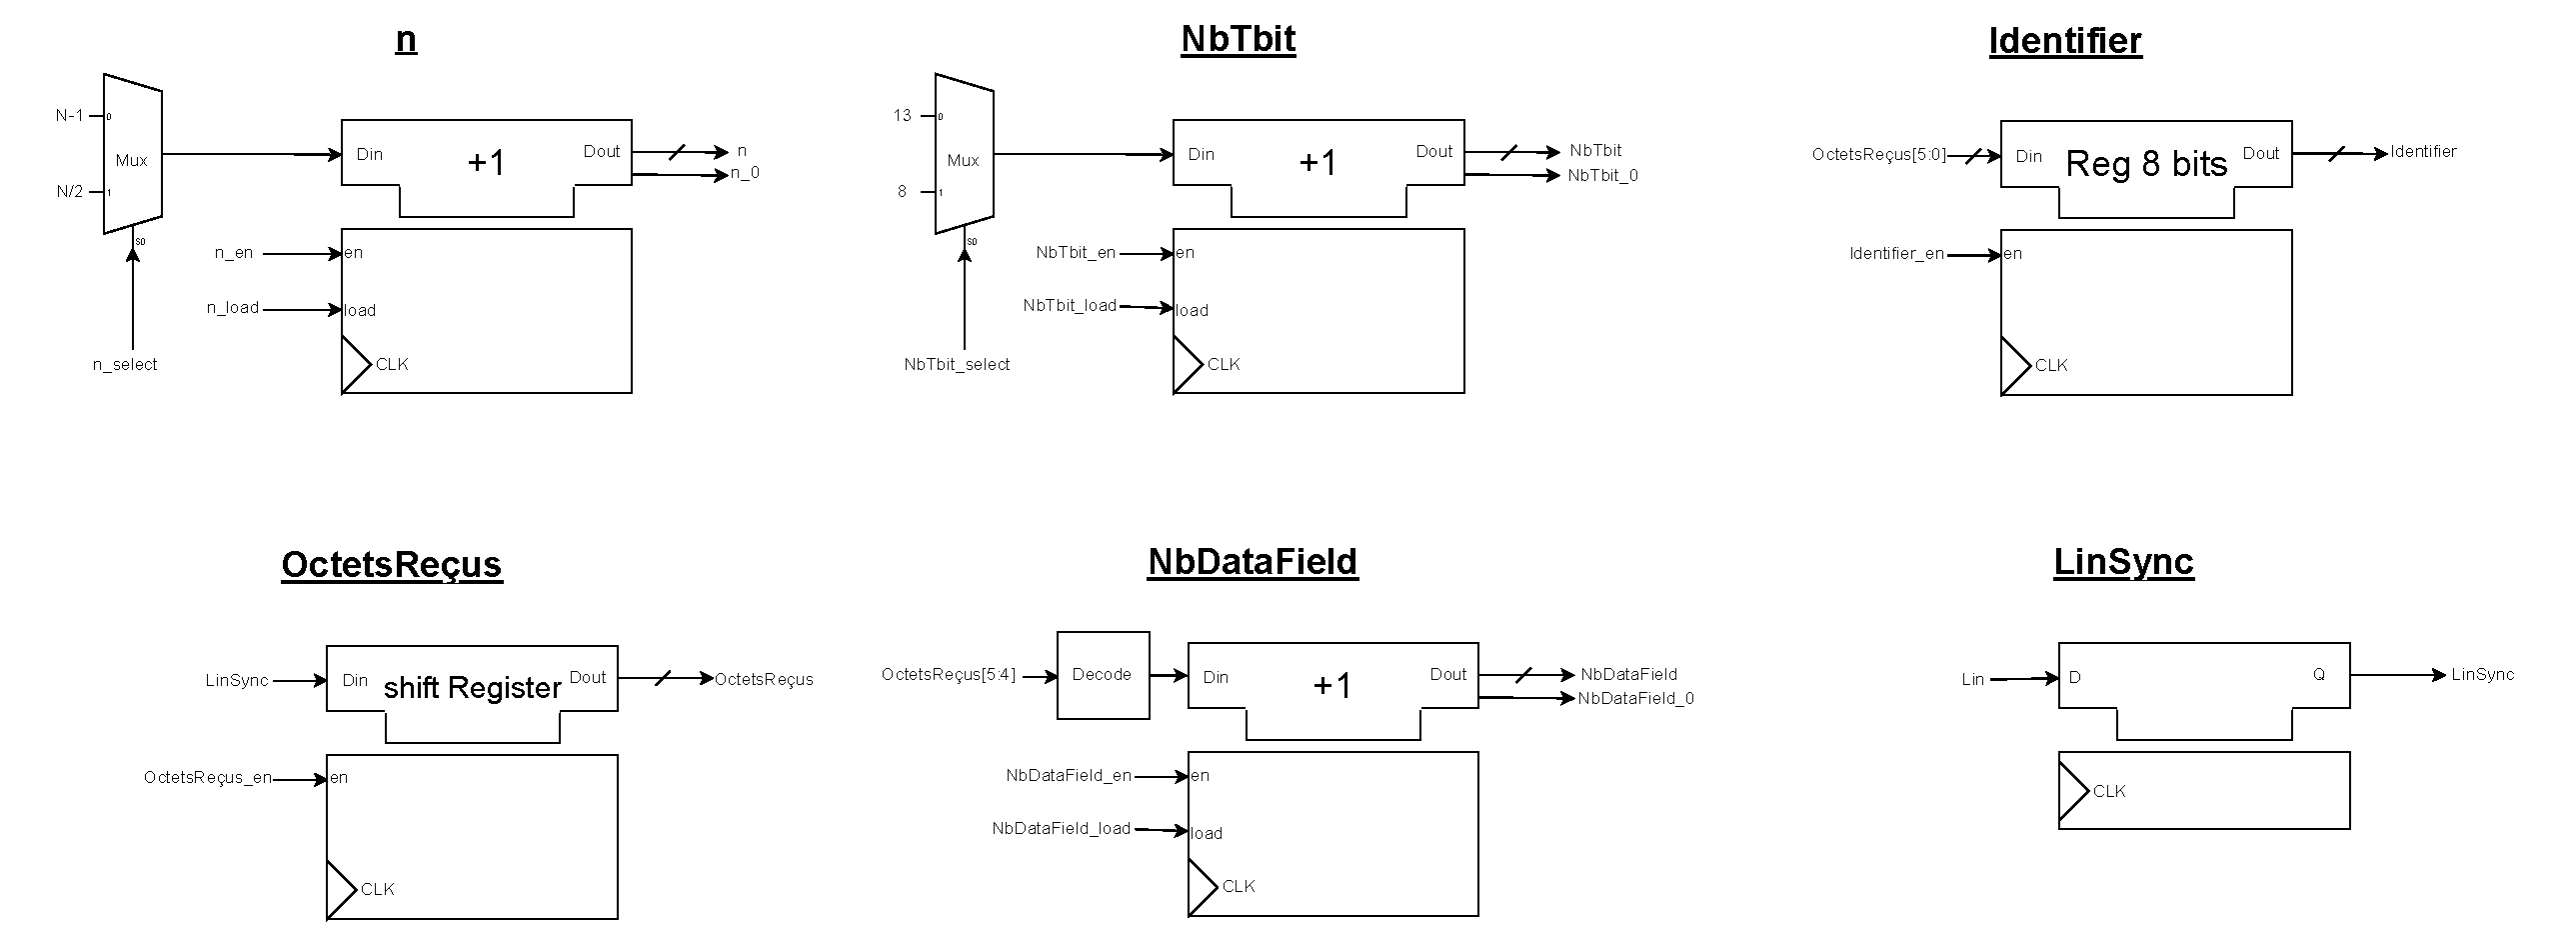
\includegraphics[width=0.95\linewidth]{images/inter/Structure_Reception_trame.pdf}
    \caption{Structure opérative du bloc de réception de trame}
    \label{fig:reception_structure}
\end{figure}

La partie commande est implémentée sous forme d’un \textbf{automate séquentiel}, représentant les différents états de réception d’une trame LIN.

\begin{figure}[H]
    \centering
    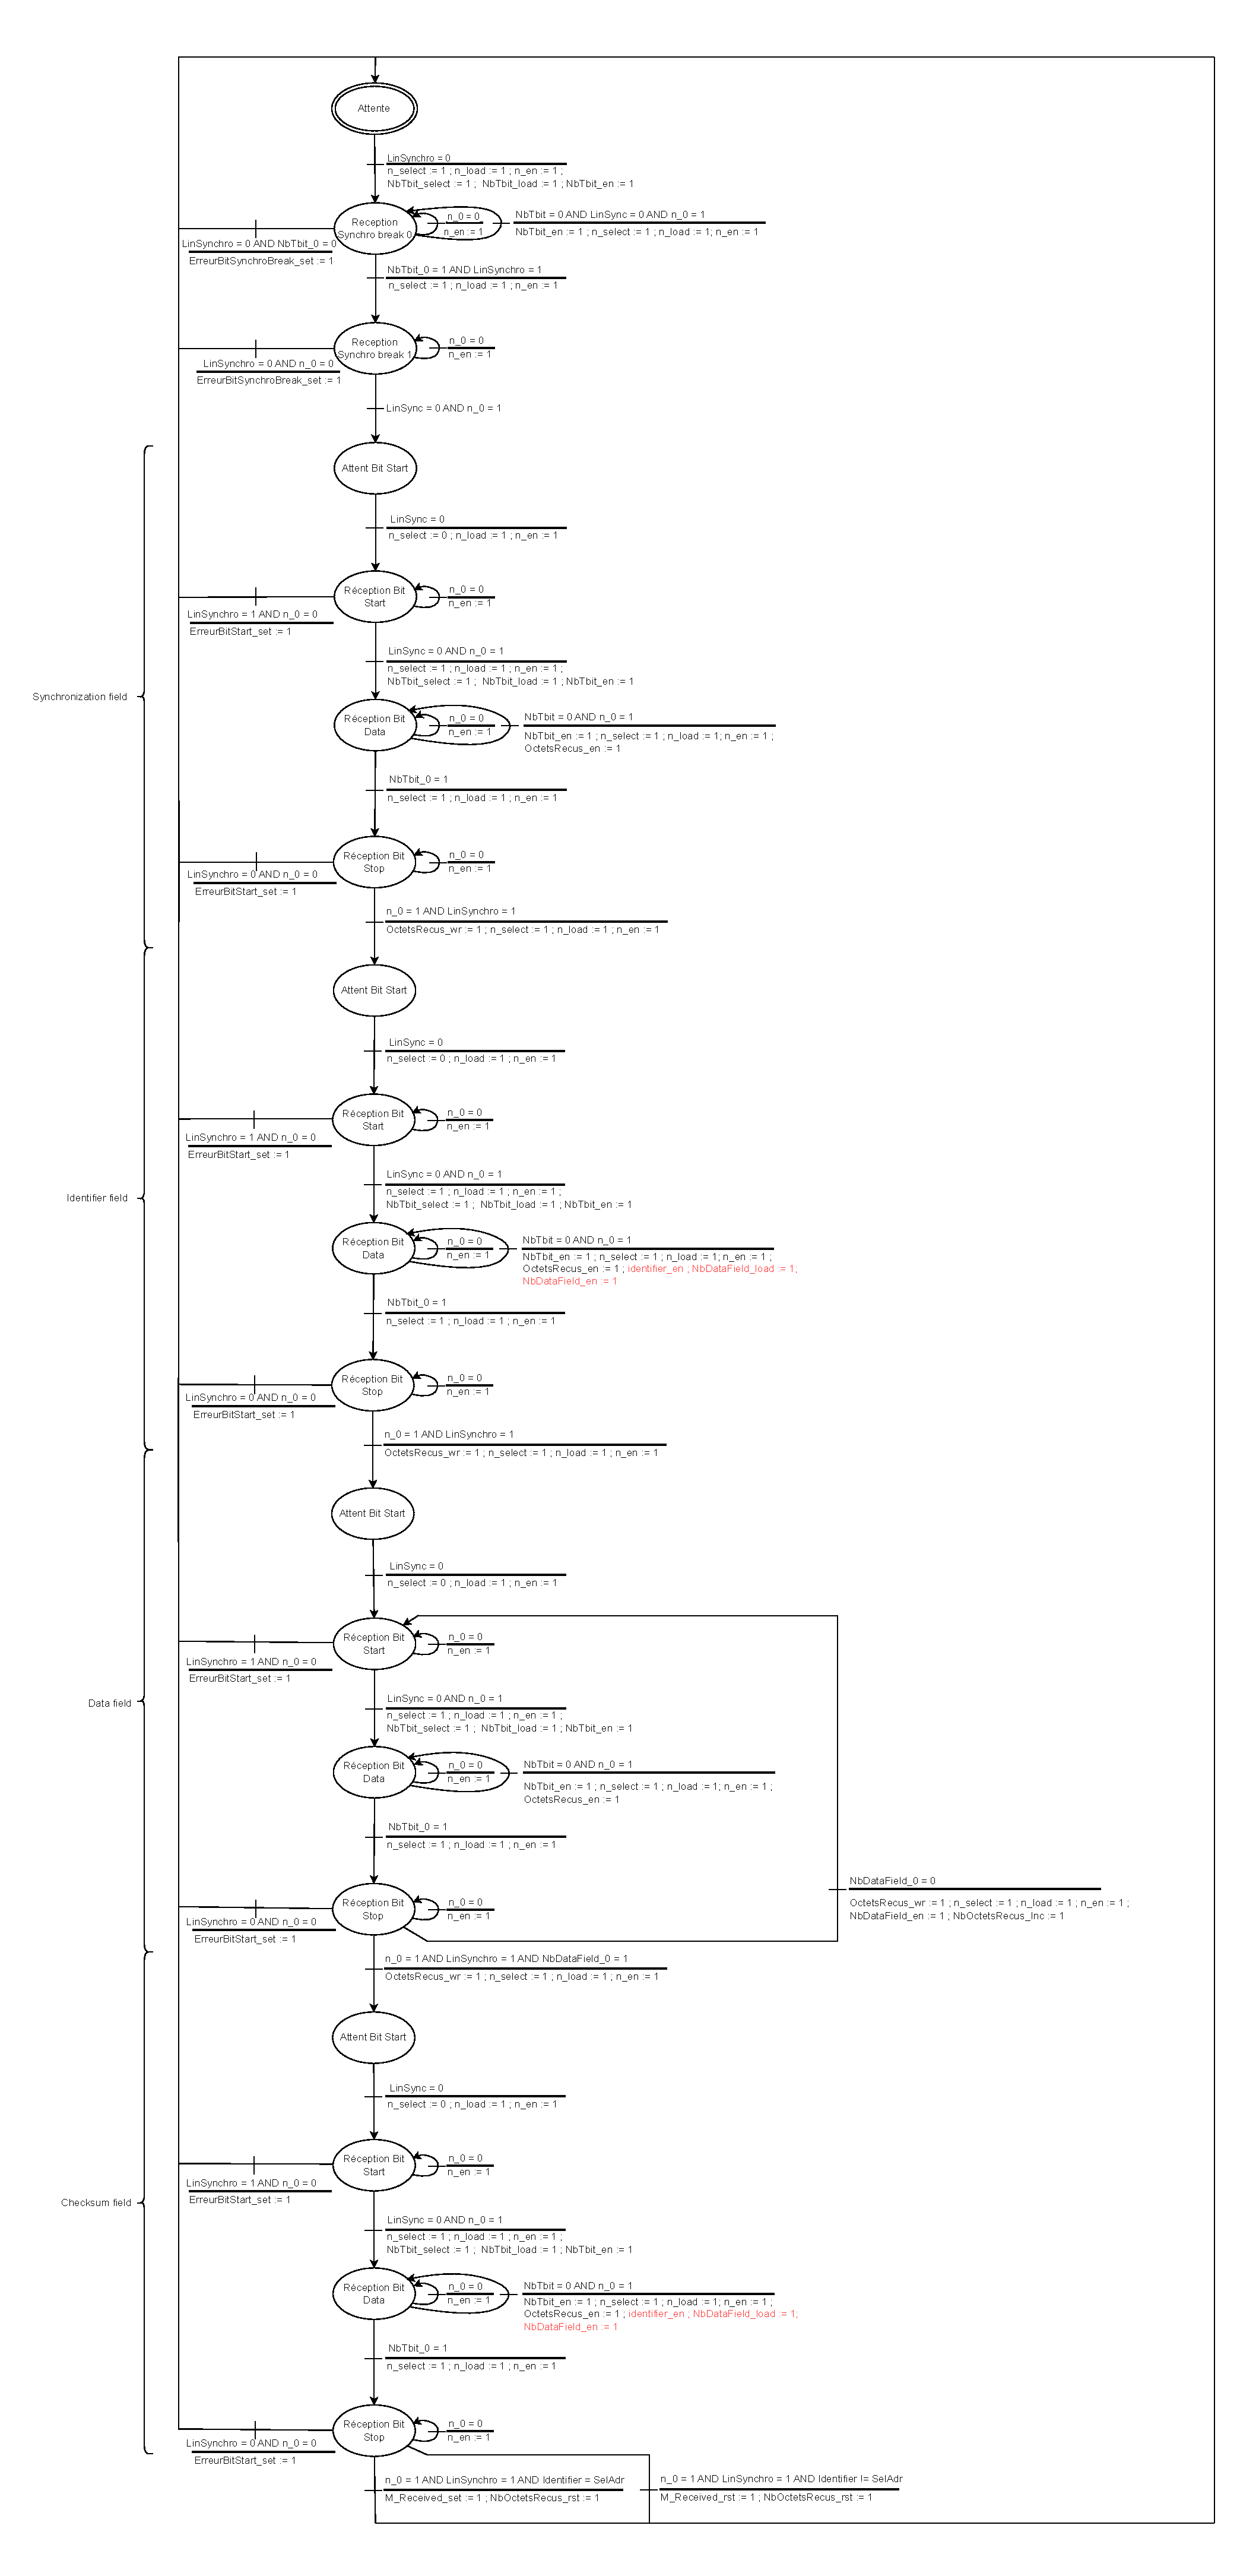
\includegraphics[width=0.6\linewidth]{images/inter/Automate_Reception_trame.pdf}
    \caption{Automate de réception de trame LIN}
    \label{fig:automate_reception}
\end{figure}

\subsection*{Description de l’automate}

L’automate décrit la séquence d’opérations depuis l’attente du signal de début jusqu’à la validation de la trame complète.  
Il gère successivement les phases suivantes :
\begin{itemize}
    \item \textbf{Attente et détection de break de synchronisation}
    \item \textbf{Réception du champ de synchronisation}
    \item \textbf{Réception de l’identifiant et des données}
    \item \textbf{Vérification du checksum et validation de la trame}
\end{itemize}

Les erreurs de synchronisation ou de bits sont détectées via des indicateurs spécifiques (erreurs de start, stop, ou synchro).  
Ce fonctionnement correspond à une \textbf{machine de Mealy}, dans laquelle les sorties dépendent à la fois des états internes et des entrées instantanées.

\begin{figure}[H]
    \centering
    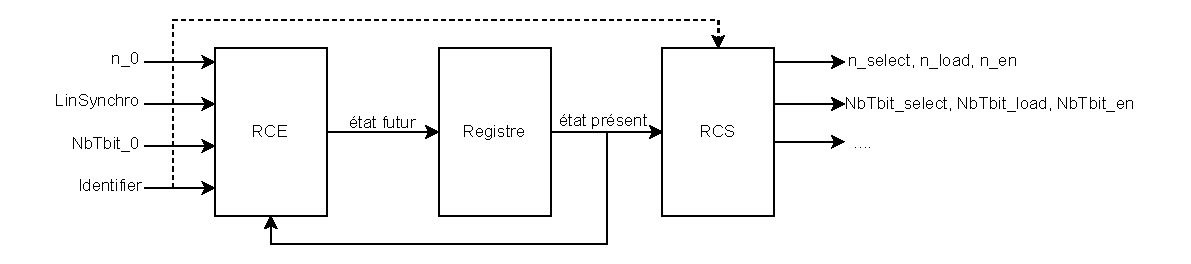
\includegraphics[width=0.8\linewidth]{images/inter/MEALY_Reception_trame.pdf}
    \caption{Machine de Mealy – Unité de commande de réception de trame}
    \label{fig:mealy_reception}
\end{figure}

\subsection{Architecture de l’Interface Microprocesseur}

Ce bloc gère les échanges entre le microprocesseur et les registres internes du système.  
Il coordonne la lecture et l’écriture des données, ainsi que la signalisation de fin de réception.

\begin{center}
\renewcommand{\arraystretch}{1.2}
\small
\begin{tabularx}{\textwidth}{|c||c|c|X|}
\hline
\textbf{Signal} & \textbf{Sens} & \textbf{Nature} & \textbf{Rôle fonctionnel} \\ \hline
D\_BUS & Bidirectionnel & Données & Bus de communication principal \\ 
CS & Entrée & Commande & Sélection du circuit \\ 
RW & Entrée & Commande & Lecture ou écriture \\ 
CD & Entrée & Commande & Sélection entre commande et données \\ 
RESET & Entrée & Commande & Réinitialisation du système \\ 
FRAME\_RECEIVED & Sortie & Indicateur & Signal de fin de réception \\ 
CLK & Entrée & Synchronisation & Horloge du système \\ 
STATE\_IN & Entrée & Données & État interne du système \\ 
DEC\_COUNT & Sortie & Commande & Décrémentation du compteur FIFO \\ 
STATE\_RST & Sortie & Commande & Réinitialisation de l’état \\ 
DATA\_IN & Entrée & Données & Donnée issue de la FIFO \\ 
DATA\_SEL & Sortie & Commande & Sélection du type de donnée affichée \\ 
\hline
\end{tabularx}
\end{center}

\begin{figure}[H]
    \centering
    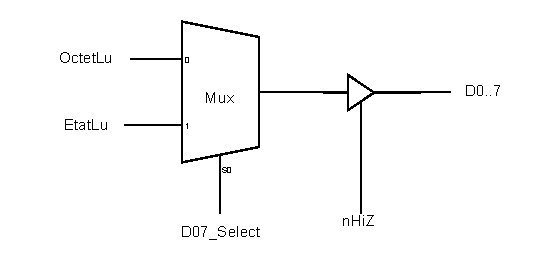
\includegraphics[width=0.8\linewidth]{images/inter/Structure_Interface_Micro.pdf}
    \caption{Structure opérative de l’interface microprocesseur}
    \label{fig:micro_interface}
\end{figure}

L’unité de commande correspondante est également décrite par un automate de type Mealy :

\begin{figure}[H]
    \centering
    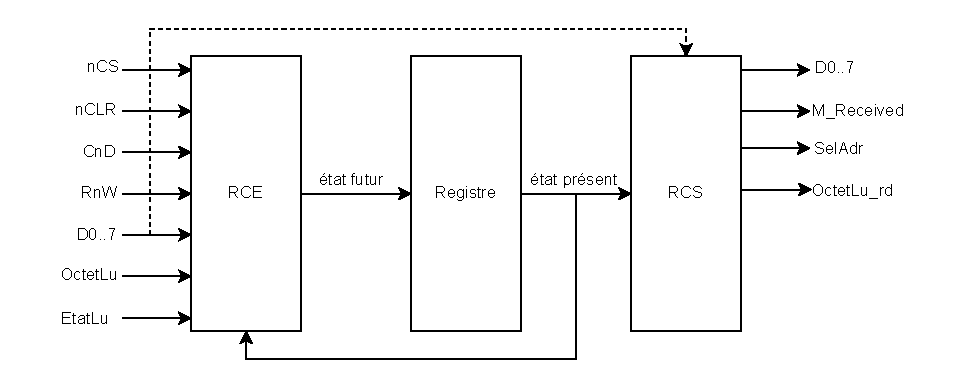
\includegraphics[width=0.8\linewidth]{images/inter/MEALY_Interface_Micro.pdf}
    \caption{Machine de Mealy – Interface microprocesseur}
    \label{fig:mealy_micro}
\end{figure}

\subsection{Architecture de la Mémoire FIFO}

La FIFO assure le stockage temporaire des octets reçus.  
Étant de complexité limitée, elle est décrite directement sous forme structurelle.

\begin{center}
\renewcommand{\arraystretch}{1.2}
\small
\begin{tabularx}{\textwidth}{|c||c|c|X|}
\hline
\textbf{Signal} & \textbf{Sens} & \textbf{Nature} & \textbf{Rôle fonctionnel} \\ \hline
DATA\_IN & Entrée & Données & Données reçues à stocker \\ 
WRITE & Entrée & Commande & Validation d’écriture \\ 
RESET & Entrée & Commande & Réinitialisation du contenu \\ 
DATA\_OUT & Sortie & Données & Données lues \\ 
READ & Entrée & Commande & Validation de lecture \\ 
\hline
\end{tabularx}
\end{center}

\begin{figure}[H]
    \centering
    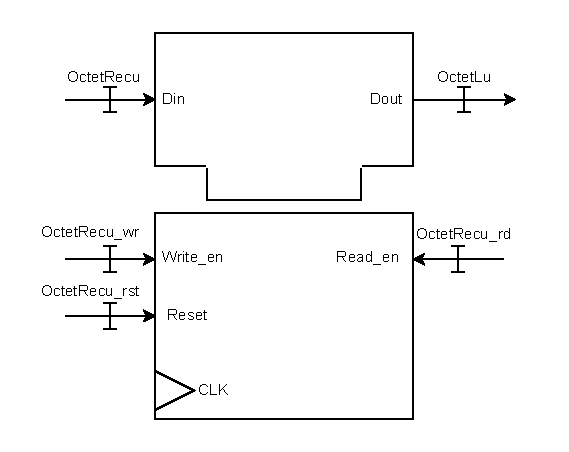
\includegraphics[width=0.8\linewidth]{images/inter/Implementation_FIFO.pdf}
    \caption{Implémentation structurelle de la mémoire FIFO}
    \label{fig:fifo}
\end{figure}

\subsection{Implémentation du Registre d’État}

Le registre d’état regroupe les informations relatives aux erreurs, au nombre d’octets reçus et à la validation des trames.

\begin{figure}[htbp]
    \centering
    \begin{subfigure}[b]{0.49\textwidth}
        \centering
        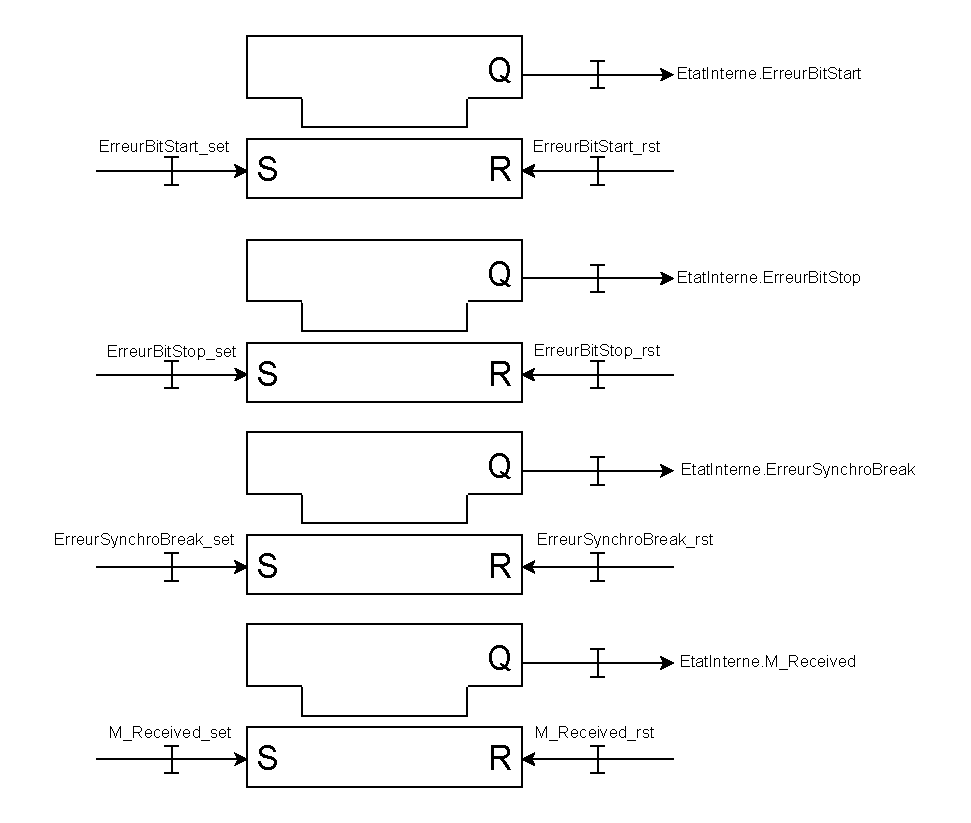
\includegraphics[width=\textwidth]{images/inter/Implementation_ETAT_Erreur.pdf}
        \caption{Mémorisation des erreurs détectées}
    \end{subfigure}
    \hfill
    \begin{subfigure}[b]{0.49\textwidth}
        \centering
        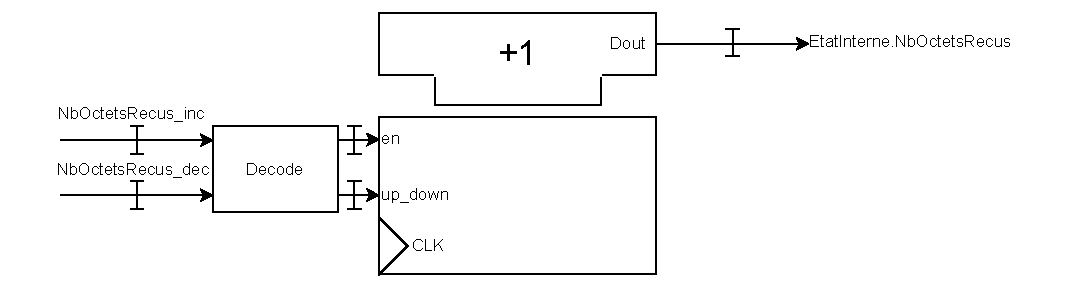
\includegraphics[width=\textwidth]{images/inter/Implementation_ETAT_NbOctets.pdf}
        \caption{Comptage des octets reçus}
    \end{subfigure}
    \caption{Implémentation structurelle du registre d’état au niveau RT}
    \label{fig:etat_impl}
\end{figure}
